% -*- coding: utf-8 -*-

\section{Algorithms}
\label{algorithms}

\subsection{Introduction}
In this section I will go into high-level detail about the principal problems that are to be solved in this project, as well as the algorithms that I have used to solve them. With each algorithm I will include an explanation of their use, an analysis of the algorithms run-time. 

\subsection{Overlap}
\label{overlap}
In order to be able to use the Rectangular Swept Sphere (RSS) in ProGAL framework, it is paramount that I must find a fast way to detect when 2 RSS' are overlapping, so that it can be decided whether a fold of the protein should go ahead or not. In the following I will describe the methods I have used to check whether or not two RSS' are overlapping.

\subsubsection{Approach}
In the algorithm I have chosen to implement, I will prefer to report a possible overlap where there might not be one, instead of failing to report a possible overlap. While this may give a performance penalty, it is critically important that illegal folding of the proteins are not accepted. 

The algorithm is split into 2 phases: The minimum distance test and the axis separation test. The first test finds the minimum distance between the rectangles of the RSS', which quickly can report an intersection, but doesn't always work, the second test finds out whether there is an axis separating the 2 RSS' (in which case they cannot intersect), which takes longer time than the first, but which always gives a correct answer. 

\subsubsection{Minimum distance}

\begin{figure}
\centering
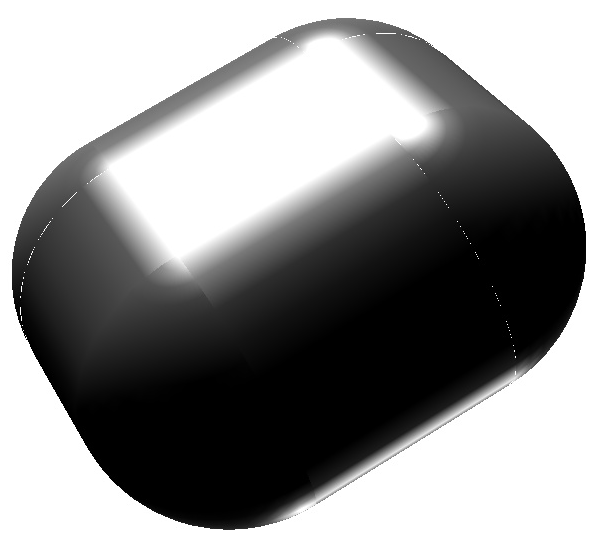
\includegraphics[width=0.5\textwidth]{figures/normalInter}
\caption{\label{normal-inter}An example of 2 RSS overlapping}
\end{figure}

\begin{figure}
\centering
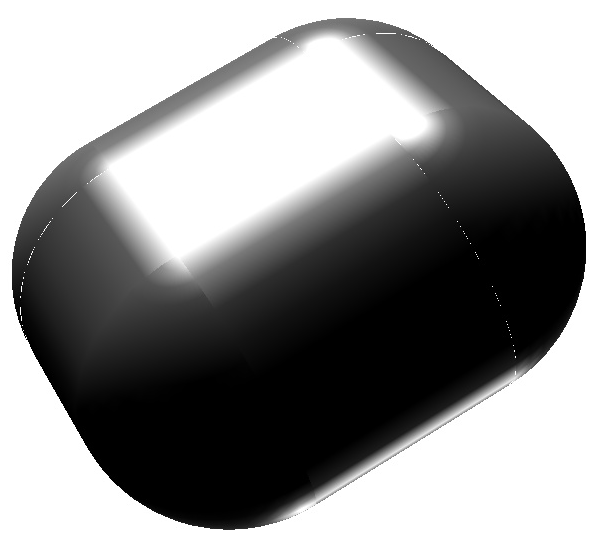
\includegraphics[width=0.5\textwidth]{figures/sepAxis}
\caption{\label{sep-Axis}Where one of the RSS lies above and ``inside'' the other}
\end{figure}

In the following let minDist(rec(A), rec(B)) be the minimum distance between the rectangles of RSS A and B, radius(A) is the radius of A.\\

One approach to check if 2 RSS', A and B, overlap, is to check the minimum distance between their rectangles. It is clear that if minDist(rec(A), rec(B)) $<=$ Radius(A) + radius(B) - see figure \ref{normal-inter} for an illustration, then A and B must overlaps. This is the approach found in \cite{Larsen99fastproximity}.

The problem then becomes one of finding the 2 closest points between rec(A) and rec(B), and calculating the distance.
Given that the rectangles do not overlap, then the possible configurations of the closest points are, according to section 4.2.1 of \cite{Larsen99fastproximity}:
\begin{enumerate}
\item Both of the points lie on an edge. This is the situation illustrated in figure \ref{normal-inter}.
\item One of the points lie in the interior of one of the rectangles (where the other point lies is irrelevant). 
\end{enumerate}

\subsection{The points lie on 2 edges}
\label{minimumDistance}
Since we are only interested in the smallest minimum distance between pairs of edges, it is clear that we only need to calculate the minimum distance between the edges that are closest to each other, all other edges will by definition be further away. The approach in my implementation is the one described in \cite{larsen00fast} and \cite{Larsen99fastproximity}, where the authors exploit the properties of Voronoi diagrams\footnote{For a formal description of Voronoi diagrams see \cite{compgeom:2008} Chapter 7} in order to quickly decide which pair of edges might be closest together. For a more detailed justification of this, see \cite{larsen00fast} section 4.2 and \cite{Larsen99fastproximity} section 4.3.1 - particularly Lemma 1. 

\begin{figure}
\centering
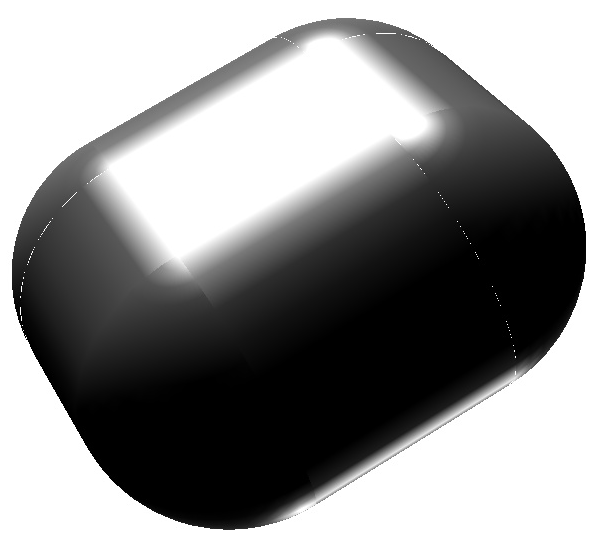
\includegraphics[width=\textwidth]{figures/vorCheap}
\caption{\label{vor-cheap}An illustration of the cheap Voronoi diagram method (2d for simplification). The letters indicate which edges are closest to that area. Areas which multiple letters will be checked by multiple edges. For instance, the edges of RSS2 that either lie completely, or partially in area 3 will be checked by both RSS1's edge a and d. The edges of RSS2 that lies entirely within area 5 will only be checked by RSS1's edge d.}
\end{figure}

Fortunately I do not need to calculate the Voronoi diagram in order to detect which Voronoi cell an edge/line-segments lies in. Let E be the edge whose closest edges we wish to find, \textbf{n} be vector perpendicular to E, then the face defined by -\textbf{n} and a point on E will define the half-plane D. All edges/line-segments that lies, wholly or partly, within D are candidates for the closest edge, as described in \cite{larsen00fast}. Using this approach, instead of explicitly calculating the Voronoi diagram, has the disadvantage that an edge might lie in multiple half-planes. However, even in the worst case this would mean that 8 checks would have had to be made, which still is better than doing 16 checks. See figure \ref{vor-cheap} for an example of this.

The problem then becomes one of finding the minimum distance between 2 line-segments in 3 dimensions, and then returning the smallest of these values. If no possible candidates are found, then infinity is returned.

If the RSS' overlap, or if one of the points closest to one of the rectangles lies in the interior, or the minimum distance between the 2 RSS is greater than the maximum radius, then it becomes necessary to run the separating axis test, which is discuss below.

\subsection{Separating axis test}
\label{sepAxis}

In order to take care of the cases where 2 rectangles either overlap or where the closest point lies inside the interior of the rectangles, I have to do an Axis-separation check, as described in \cite{237244}. The gist of the Axis-separation test is ``that two disjoint convex polytopes in 3-space can always be separated by a plane which is parallel to a face of either polytope, or parallel to an edge from each polytope'' (\cite{237244}, section 5, page. 8).

The Axis-separation test described in \cite{237244} was designed to work on Oriented Bounding Boxes (OBB's), and takes care of rectangle to rectangle axis test as a degenerate, and faster, case (\cite{237244}, section 5).

\subsubsection{Order of Minimum distance and Axis separating test}
\label{minAxisOrder}
An important question is whatever the minimum distance test should be run first, followed by axis-seperation is optimal, or if it might be better just to run the axis separation test.

It is important to understand the purpose of the methods, and their exiting condition, the cases that causes them to exit their test at the earliest juncture, and the cases that makes makes them do the most work:

\begin{figure}
\centering
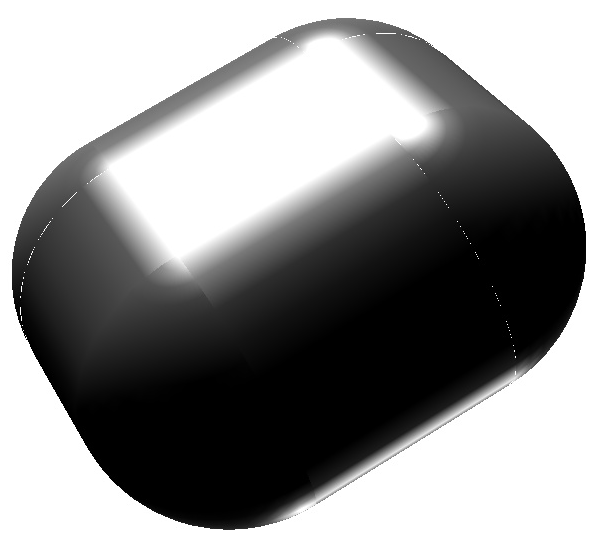
\includegraphics[width=\textwidth]{figures/vorCheap}
\caption{\label{parallel} An illustration of where one RSS lies above, and inside the other RSS.}
\end{figure}

\subsubsection{Minimum distance}
\begin{description}
\item[Purpose:] The minimum distance algorithm finds the minimum distance between edges.
\item[Exiting condition:]The exiting condition of the algorithm is when it has either checked all edges for minimum distance, or when it finds a minimum distance that is smaller than the combined radius of the RSS'. If the algorithm returns with a positive, then we know that the 2 RSS' intersect, but if it returns with a negative, then we do not know whether the 2 RSS' overlap or not. The algorithm favours the cases where the 2 RSS' might overlap.
\item[Best case:] The first edge is closer than the combined radius of both RSS' - the test stops immediately.
\item[Worst case:] All the edges are tested, but the found distance is greater than the combined radius. Such a case occurs when the 2 RSS' do not overlap.
\item[Does not handle:] This algorithm cannot handle cases where one of the RSS lies ``above'' or ``below'' the other (in the plane generated by the second's RSS' rectangle). See figure \ref{parallel} for an illustration of the case.
\end{description}

\subsubsection{Axis-separation test}
\begin{description}
\item[Purpose:] The axis separation algorithm tries to find an axis that separates the 2 RSS'. 
\item[Exiting condition:] The axis-separation test terminates either when it finds in which the 2 rectangles are disjoint, or after having run all axis-tests. For the algorithm to be valid, the created RSS should therefore contain all the points - while its quality should be measured in how tight the fit is.
\item[Best case:] The first axis test shows that the 2 RSS' are disjoint, and the algorithm terminates. 
\item[Worst case:] The 2 RSS' are not disjoint, and so all 15 axis-tests (See \ref{sepAxis} for more information) have to be made.
\item[Does not handle:] Axis-separation test handles all cases.
\end{description}

It is thus clear that the worst case where RSS A overlaps with RSS B in B's interior - since this case is not handled by the minimum distance test, and the Axis-separation test will have to do all 15 tests. From this it is clear that the cases we belive to be most common case should decide the optimal order. 

If we think that it is likely that a RSS will lie in the interior or another (either overlapping the other, or lying above or below the RSS' rectangle) or that RSS' will only intersect in rare cases, then it will be a better choice to only run the Axis-separation test. If, on the other hand, we believe RSS' are unlikely to lie above/below each others rectangle, and will often intersect, then the minimum distance algorithm, followed by the Axis-separation test will be better.

Since in the context of folding proteins are interested in being told that a fold is illegal as soon as possible (so that the next fold can be tested\footnote{In a BVH, and thus in practice, we furthermore have the case that a detected overlap will lead to further tests - making it very important that cheap collision tests are possible}), I think that first running the Minimum distance algorithm, and then the Axis-separation test would improve the run-time in most instances, instead of only running the Axis-separation test.

\subsection{Creating RSS from multiple points}
In order for the RSS to be a useful data-structure, it is clear that I have to find an algorithm that given a set of points, constructs a RSS that contains all of the points. The primary quality measurement should be the tightness of the volume.

In the implemented algorithm I uses the properties of the eigen vectors from the covariance matrix. The idea is to use the eigen vectors to decide the vectors for the longest side (the eigen-vector with the greatest length), the second longest side (the eigen-vector with the second greatest length) and the radius (the eigen-vector with the smallest length). For each of these vectors v, I then create the plane p that goes through origo with v, project all the points onto p, and then finds the greatest distance between all pairs of projected points, which then is used as the the length of v.
\hide{
While I find the pair with the greatest distance for the 3 vectors, I also find the point that lies between these two points. Since these points are likely to be different, find the absolute difference of the 3 points 3 coordinates, and add these values to their respective vector's length. The center point can then be chosen arbitrarily.
}
\begin{algorithm}[H]
  \caption{CreateRSSContainingPoints}
  \label{create-algo}
  \SetKwData{covar}{CovarianceMatrix}
  \SetKwData{eigen}{EigenVectors}
  \SetKwData{threedeeRec}{3dRec}
  \SetKwData{return}{return}
  \SetKwData{p}{p}
  \SetKwInOut{Input}{input} \SetKwInOut{Output}{output}
  \dontprintsemicolon
  \Input{A set P of n points in 3 dimensions}
  \Output{A RSS that contains all points in P}
  \covar $\gets$ makeCovarainceMatrix(P)\;
  \eigen $\gets$ getEigen(\covar) \;
  \eigen $\gets$ sort(\eigen) \;
  (longest, centerPoint1) $\gets$ getLongestDistance(\eigen[2], points) \;
  (middle, centerPoint2) $\gets$ getLongestDistance(\eigen[1], points) \;
  (shortest, centerPoint3) $\gets$ getLongestDistance(\eigen[0], points) \;
  centerPoint $\gets$ points.getCenteroid() \;
  subtract shortest from longest and middle
  \threedeeRec $\gets$ 3dRec(centerPoint1, \eigen[2].scaledTo(longest), \eigen[1].scaledTo(middle)) \;
  \return RSS(\threedeeRec, shortest) \;
\end{algorithm}

\subsubsection{Asymptotic Runtime}
The subroutine that finds the covariance matrix for algorithm \ref{create-algo} runs in $O(n)$. The subroutine that finds the distance between every pair of of points runs in $O(n^2)$, and everything else runs in constant time. Thus the algorithm must have an asymptotic run-time of $O(n^2)$.

\subsection{Algorithm to create a RSS containing 2 RSS'}
In order to combine  2 RSS', rss1 and rss2, I take all the points that define the RSS' and then create a new RSS from the combined pointset. 

\begin{algorithm}[H]
  \caption{CombinedRSS}
  \label{combine-algo}
  \SetKwData{points}{pointsSet}
  \SetKwData{crss}{CombinedRSS}
  \SetKwData{return}{return}
  \SetKwInOut{Input}{input} \SetKwInOut{Output}{output}
  \dontprintsemicolon
  \Input{2 RSS' rss1 and rss2}
  \Output{A RSS that contains both RSS'}
  Initialize \points \;
  Add points(rss1) and points(rss2) to \points \;
  \return CreateRSSContainingPoints(\points) \;
\end{algorithm}

\subsubsection{Asymptotic Runtime}
It is clear that algorithm \ref{combine-algo} must run in $O(n^2)$, where n is the combined number of pionts in both RSS1 and RSS2. 

%\subsection{Non-axis aligned rectangle}

\subsection{Efficiency}
I will in the following assume that all RSS are created in order to contain a point set (this is a reasonable assumption in practice). Let a normal RSS be an RSS that have been created so that all the points in the point set are contained in an OBB inside the RSS (i.e. no points lie in the half-cylinder part on the edges of the RSS). \Sfixme{Make illustration} 

From \ref{rss} it is clear that a normal RSS will essentially create a Oriented Bounding Box around the points, together with 2 cylinders around the edges. From this it is clear that if RSS are ever to be more efficient than OBB, then there must be a way to use a property of the RSS that the OBB's do not have. 

The only real property that the RSS has that the OBB does not, is the radius. This is what we are trying to exploit in the minimum distance check. As detailed in the Results section, this exploit does not lead to greatly improved run time, and it is therefore likely that a RSS with a larger volume than an OBB will never be more efficient. \Sfixme{These 2 last subsections are suspect}

\subsection{Optimized volume} 
\begin{figure}
\centering
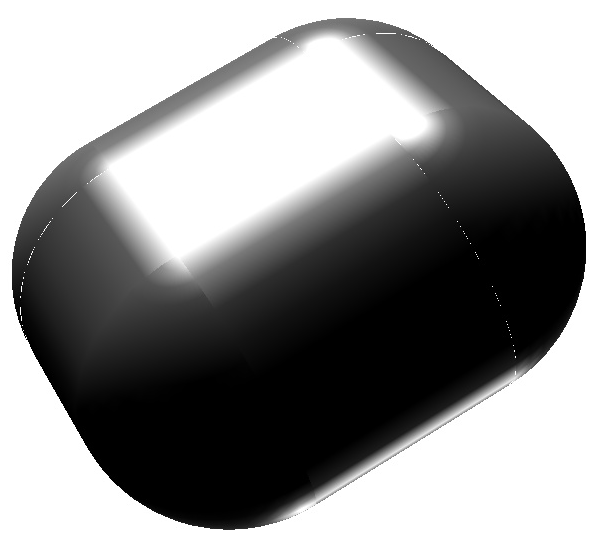
\includegraphics[width=0.5\textwidth]{figures/normalInter}
\caption{\label{optimized-volume}An example of an optimized volume, where the [Rim has been taken into use]}
\end{figure}

Since we in the Minimal distance check, makes sure that the distance between the 2 rectangles is less than the combined radius of the 2 RSS' i.e. if any part of the 2 RSS' intersect - also the part that does not lie above or below the RSS' rectangle. From this it is apparent that points could be placed outside the rectangle, but inside the Outer RSS, then the volume of the RSS could, at least in certain cases, become smaller. Finding this optimized volume would most likely take more time than algorithm \ref{create-algo}, and it unknown how much faster the overlap function would become, so it is likely worth a research project of itself. \Sfixme{Should I really mention this - is there a better way writing this section - most likely there is}

\subsection{Conclusion}
I have in this section presented the main problem that my algorithms are trying to solve - to find out whether 2 RSS' overlap, and how to create a new RSS that will contain all the points of 2 other RSS'. I have presented both algorithms on both high- and low-level, and have at the end discussed how to minimize the volume by using the rim optimally, discussed how the RSS is unlikely to become more efficient than the OBB.
